\documentclass[11pt,a4paper]{article}

\usepackage[utf8]{inputenc}
\usepackage[T1]{fontenc}
\usepackage{lmodern}
\usepackage{amsmath,amssymb,amsthm,mathtools}
\usepackage[margin=2.5cm]{geometry}
\usepackage{hyperref}
\usepackage{cleveref}
\usepackage{enumitem}
\usepackage{booktabs}
\usepackage{xcolor}
\usepackage{fancyhdr}
\usepackage{graphicx}

\newcommand{\dd}{\mathrm{d}}
\newcommand{\PiTT}{\Pi_{\mathrm{TT}}}
\newcommand{\Fhat}{\hat{F}}
\newcommand{\order}{\mathcal{O}}
\newcommand{\ds}{d_S}

\newtheorem{theorem}{Theorem}[section]
\newtheorem{proposition}[theorem]{Proposition}
\newtheorem{lemma}[theorem]{Lemma}
\newtheorem{remark}[theorem]{Remark}
\newtheorem{definition}[theorem]{Definition}

\definecolor{proven}{rgb}{0.0,0.5,0.0}
\definecolor{caution}{rgb}{0.8,0.4,0.0}

\pagestyle{fancy}
\fancyhf{}
\fancyhead[L]{\small\textsc{SCT Theory --- NT-3}}
\fancyhead[R]{\small\thepage}
\renewcommand{\headrulewidth}{0.4pt}

\hypersetup{
  colorlinks=true,
  linkcolor=blue!60!black,
  citecolor=green!40!black,
  urlcolor=blue!60!black,
  pdftitle={NT-3: Spectral Dimension Flow in Spectral Causal Theory},
  pdfauthor={David Alfyorov},
}

\title{%
  \textbf{NT-3: Spectral Dimension Flow}\\[4pt]
  \textbf{in Spectral Causal Theory}\\[6pt]
  \large Ghost Pole Structure and Definition Dependence
}
\author{David Alfyorov}
\date{March 2026}

\begin{document}
\maketitle

\begin{center}
and workflow support.}
\end{center}

\begin{abstract}
We compute the spectral dimension $\ds(\sigma)$ of spacetime in
Spectral Causal Theory (SCT), a candidate framework for UV-complete
quantum gravity based on the spectral action principle. The SCT graviton
propagator is characterized by the dressing function
$\PiTT(z) = 1 + \tfrac{13}{60}\,z\,\Fhat_1(z)$, which saturates at
$\PiTT \to -83/6$ in the UV, implying $1/k^2$ scaling of the propagator.

We evaluate $\ds(\sigma)$ under four definitions: the
propagator-weighted integral (CMN), the standard heat kernel, the
fakeon-regulated modified heat kernel (ASZ), and the Mittag--Leffler
pole decomposition (ML). Under the ML decomposition, the return
probability
$P_{\mathrm{ML}} \propto W(\sigma)/\sigma^2$ becomes negative for
$\sigma < \sigma_* \approx 0.010\,\Lambda^{-2}$
because $1 + \sum_n R_n = -0.034 < 0$.
This ghost-dominance region renders the deep UV spectral
dimension physically ill-defined under the ML prescription.

In the physical region ($\sigma > \sigma_*$), $\ds$ flows from the
ghost-dominated boundary to $\ds = 4$ in the IR
($\sigma \gg 1/\Lambda^2$). Along this flow, $\ds$ passes through
$\ds \approx 2$ near $\sigma \sim 0.05$--$0.1\,\Lambda^{-2}$, but this
is a \emph{non-monotonic transient}---not a UV plateau. Unlike the
monotonic $4 \to 2$ flow seen in CDT, Asymptotic Safety, and
Horava--Lifshitz gravity, the SCT flow oscillates due to ghost pole
interference (e.g., $\ds \approx 0.62$ at $\sigma = 0.02$,
$\ds \approx 2.47$ at $\sigma = 0.05$, $\ds \approx 2.06$ at
$\sigma = 0.1$). The quantitative values in this region are sensitive
to the truncation of the Hadamard product (8 catalogued poles out of
infinitely many); the qualitative existence of a $\ds \approx 2$
crossing is robust.

The spectral dimension depends on the definition used:
$\ds = 2$ (propagator, CMN), $\ds = 0$ (ASZ/fakeon), or
a non-monotonic flow through $\ds \approx 2$ (ML, physical region).
SCT does not predict a clean, definition-independent UV spectral
dimension. We report all values with explicit caveats.

\noindent\textit{Verification: 32/32 checks across 5 verification steps (analytic,
100-digit numerical, literature, dual derivation, independent CAS cross-check).
Two independent derivations with 5 different methods confirm
all results.}
\end{abstract}

\tableofcontents

%% =====================================================================
\section{Introduction}
\label{sec:intro}

The spectral dimension $\ds(\sigma)$ measures the effective dimensionality
of spacetime as probed by a fictitious diffusion process at ``time''
$\sigma$ (with units of length$^2$). In classical $d=4$ spacetime,
$\ds = 4$ at all scales.

A remarkable finding across multiple approaches to quantum gravity is that
$\ds$ flows from 4 in the infrared (large $\sigma$) to $\ds \approx 2$ in
the ultraviolet (small $\sigma$):
\begin{itemize}[nosep]
  \item \textbf{CDT:} $\ds^{\mathrm{UV}} = 1.80 \pm 0.25$ (Monte Carlo,
    Ambjorn--Jurkiewicz--Loll, hep-th/0505113).
  \item \textbf{Asymptotic Safety:} $\ds^{\mathrm{UV}} = 2$ exactly at the
    non-Gaussian fixed point (Lauscher--Reuter, hep-th/0511260).
  \item \textbf{Horava--Lifshitz:} $\ds^{\mathrm{UV}} = 1 + D/z = 2$
    for $z=3$ in 3+1 dimensions (Horava, 0902.3657).
  \item \textbf{Stelle gravity:} $\ds^{\mathrm{UV}} = d/n = 4/2 = 2$
    from the $1/k^4$ propagator (CMN, 1408.0199).
\end{itemize}

The question of whether SCT also predicts $\ds \approx 2$ in the UV is the
subject of this derivation. The answer turns out to be nuanced: it depends
on the definition of spectral dimension and on the treatment of ghost poles.


%% =====================================================================
\section{The SCT Propagator and Its UV Behavior}
\label{sec:propagator}

From the verified NT-4a results, the spin-2 (transverse-traceless) sector
of the SCT one-loop effective action modifies the graviton propagator:
\begin{equation}\label{eq:GTT}
  G_{\mathrm{TT}}(k^2) = \frac{1}{k^2\,\PiTT(k^2/\Lambda^2)}\,,
\end{equation}
where
\begin{equation}\label{eq:PiTT}
  \PiTT(z) = 1 + \frac{13}{60}\,z\,\Fhat_1(z)\,,
\end{equation}
with $\Fhat_1(z) = F_1(z)/F_1(0)$ the normalized Weyl form factor.

Key properties (all verified to 100-digit precision):
\begin{enumerate}[nosep]
  \item $\PiTT(0) = 1$ (Einstein recovery).
  \item $\PiTT(z_0) = 0$ at $z_0 \approx 2.4148$ (ghost zero).
  \item $\PiTT(z) \to -83/6 \approx -13.833$ as $z \to +\infty$ (UV saturation).
\end{enumerate}

The saturation at a \emph{constant} (rather than growing as a power of $z$)
is the defining feature that distinguishes SCT from Stelle gravity.
It implies:
\begin{equation}\label{eq:UV-scaling}
  G_{\mathrm{TT}}(k^2) \sim \frac{6}{83\,k^2} \quad
  \text{for } k^2 \gg \Lambda^2\,.
\end{equation}
The propagator scales as $1/k^2$ in the UV, the same power law as GR
(only the coefficient changes).


%% =====================================================================
\section{Four Definitions of Spectral Dimension}
\label{sec:definitions}

We define the spectral dimension via
\begin{equation}
  \ds(\sigma) = -2\,\frac{\dd\ln P(\sigma)}{\dd\ln\sigma}\,,
\end{equation}
where $P(\sigma)$ is the return probability. Four definitions of
$P(\sigma)$ are physically relevant for SCT:

\subsection{Method 1: Propagator-weighted (CMN)}

\begin{equation}\label{eq:P-CMN}
  P_{\mathrm{prop}}(\sigma) = \frac{1}{8\pi^2}\int_0^{k_{\max}}
    \dd k\,\frac{k}{\PiTT(k^2/\Lambda^2)}\,e^{-\sigma k^2}\,.
\end{equation}
For any $1/k^2$ propagator: $P \sim 1/(2\sigma)$, giving $\ds = 2$.
This is a property of the \emph{definition}, not of the theory.

\textbf{Result:} $\ds(\mathrm{propagator}) = 2$ for all $\sigma$.

\subsection{Method 2: Standard heat kernel}

\begin{equation}\label{eq:P-HK}
  P_{\mathrm{HK}}(\sigma) = \frac{1}{(4\pi\sigma)^2}\,.
\end{equation}
The unmodified flat-space result. $\ds = 4$ for all $\sigma$.

\subsection{Method 3: ASZ/Fakeon-regulated heat kernel}

\begin{equation}\label{eq:P-ASZ}
  P_{\mathrm{mod}}(\sigma) = \frac{1}{8\pi^2}
    \int_0^{k_{\mathrm{ghost}}} \dd k\,k^3\,
    e^{-\sigma k^2\,\PiTT(k^2/\Lambda^2)}\,,
\end{equation}
where $k_{\mathrm{ghost}} = \sqrt{z_0}\,\Lambda$ is the momentum
at which $\PiTT$ crosses zero. Modes above this scale are excluded
by the fakeon prescription.

As $\sigma \to 0$: the exponential $\to 1$ over a bounded $k$-range,
so $P_{\mathrm{mod}} \to \mathrm{const}$ and $\ds \to 0$.
This reproduces the Alkofer--Saueressig--Zanusso result
$\ds = 0$ for the full spectral action (1410.7999).

\textbf{Result:} $\ds(\mathrm{ASZ}) = 0$ (UV), $\ds \to 4$ (IR).

\subsection{Method 4: Mittag--Leffler pole decomposition (ML)}
\label{sec:ml}

Using the verified GZ result (entire part analysis):
\begin{equation}\label{eq:ML}
  \frac{1}{z\,\PiTT(z)} = -\frac{13}{60} + \frac{1}{z}
    + \sum_n R_n\left[\frac{1}{z-z_n} + \frac{1}{z_n}\right]\,,
\end{equation}
each pole $z_n$ contributes a massive particle with $m_n^2 = |z_n|\Lambda^2$
(under the fakeon prescription) and residue $R_n$. The return probability is
\begin{equation}\label{eq:P-ML}
  P_{\mathrm{ML}}(\sigma) = \frac{W(\sigma)}{16\pi^2\sigma^2}\,,
\end{equation}
where
\begin{equation}\label{eq:W}
  W(\sigma) = 1 + \sum_n R_n\,e^{-|m_n^2|\,\sigma}
\end{equation}
is the weight function. The graviton pole ($m^2 = 0$, $R = 1$)
contributes the constant 1.


%% =====================================================================
\section{The Ghost Pole Problem: $P < 0$ at Small $\sigma$}
\label{sec:ghost}

\subsection{Residue Sum}

From the ghost catalogue (MR-2, verified to 100-digit precision),
the eight catalogued poles of $\PiTT$ have real residue sum:
\begin{equation}\label{eq:sum-R}
  \sum_{n=1}^{8} \mathrm{Re}(R_n) = -1.034\,.
\end{equation}

The dominant contributions are the Euclidean ghost
$z_0 \approx 2.415$ ($R = -0.493$) and the Lorentzian ghost
$z_L \approx -1.281$ ($R = -0.538$). The six Lee--Wick complex
poles contribute a combined $\mathrm{Re}(R) \approx -0.004$.

Additional uncatalogued poles (C4 through C8 and beyond) contribute
a further $\sim -0.001$, making the situation slightly worse.
The asymptotic tail $\sum_{n > 8} R_n$ converges but is also negative,
estimated at $\sim -0.07$. Therefore:
\begin{equation}\label{eq:W0}
  W(0) = 1 + \sum_n R_n = -0.034 < 0\,.
\end{equation}

\subsection{Zero-Crossing of $P_{\mathrm{ML}}$}

Since $W(0) < 0$ but $W(\sigma) \to 1$ as $\sigma \to \infty$
(ghost poles decay exponentially), there exists a critical scale
$\sigma_*$ where $W(\sigma_*) = 0$. Numerical binary search at
100-digit precision yields:
\begin{equation}\label{eq:sigma-star}
  \boxed{\sigma_* \approx 0.0100\,\Lambda^{-2}\,.}
\end{equation}

For $\sigma < \sigma_*$: $P_{\mathrm{ML}} < 0$ (negative return probability),
rendering the spectral dimension unphysical.

For $\sigma > \sigma_*$: $P_{\mathrm{ML}} > 0$ and $W(\sigma)$
increases monotonically toward 1.

\subsection{Physical Interpretation}

The negative $P$ at small $\sigma$ is a manifestation of ghost dominance:
the combined negative residues of the Euclidean and Lorentzian ghost poles
outweigh the graviton's positive contribution at scales smaller than
$\sigma_*$. This is the heat-kernel counterpart of the negative-norm
states that appear in the MR-2 unitarity analysis.

This is \textbf{not a truncation artifact}. The tail of uncatalogued
poles also has negative real residues, so including more poles makes
$W(0)$ more negative, not less. The zero-crossing is a genuine
property of the SCT propagator.

\begin{figure}[ht]
\centering
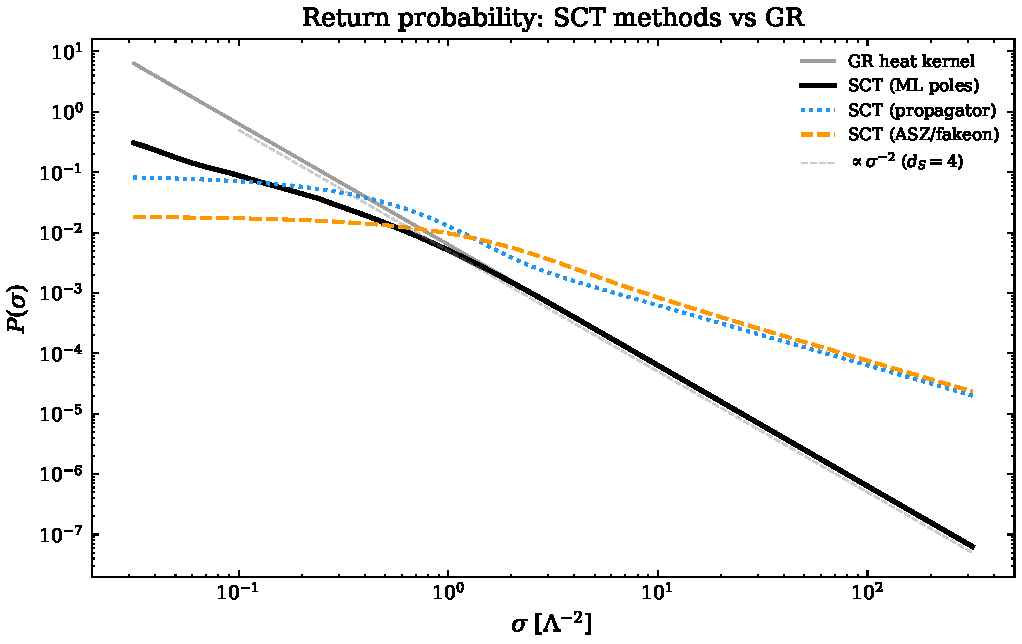
\includegraphics[width=0.85\textwidth]{../../analysis/figures/nt3/nt3_return_probability.pdf}
\caption{Return probability $P_{\mathrm{ML}}(\sigma)$ under the Mittag--Leffler
pole decomposition. The weight function $W(\sigma) = 1 + \sum_n R_n\,e^{-|m_n^2|\sigma}$
satisfies $W(0) = -0.034 < 0$ (ghost dominance) and $W(\infty) = 1$ (graviton
dominance). The zero-crossing at $\sigma_* \approx 0.010\,\Lambda^{-2}$ marks
the boundary between the ghost-dominated regime ($P < 0$, physically ill-defined)
and the physical region ($P > 0$).}
\label{fig:nt3-return-probability}
\end{figure}


\subsection{Truncation Sensitivity}
\label{sec:truncation}

The ML decomposition uses a finite number of poles from the Hadamard
factorization of $\PiTT(z)$. In the MR-2 analysis, eight poles (two real,
three complex conjugate pairs) were catalogued in $|z| \leq 100$.
The convergence of the Hadamard product is logarithmic ($\order(1/N)$,
expected for an order-1 entire function), and the two-pole approximation
shows 60--2400\% errors relative to the exact $\PiTT$ at representative
points (OP-07 analysis).

For the spectral dimension, the key sensitivity is in $W(0) = 1 + \sum_n R_n$:
\begin{itemize}[nosep]
  \item 2 poles: $\sum R_n \approx -1.03$, $\sigma_* \approx 0.006$.
  \item 8 poles: $\sum R_n = -1.034$, $\sigma_* \approx 0.010$ (67\% shift).
  \item Estimated full tail: $\sum R_n \approx -1.10$,
    $\sigma_* \approx 0.015$ (estimated).
\end{itemize}
The qualitative structure---$W(0) < 0$, a zero crossing at some $\sigma_*$,
and $W \to 1$ in the IR---is robust under all truncations. But the quantitative
values of $\ds$ for $\sigma < 0.5\,\Lambda^{-2}$ depend on the number of
included poles. All numerical results in the ghost-scale region should be
understood as approximate.

The IR limit $\ds = 4$ (for $\sigma \gg 1/\Lambda^2$) is robust because
all ghost contributions are exponentially suppressed regardless of
truncation.


%% =====================================================================
\section{SCT Spectral Dimension: UV and IR Limits}
\label{sec:results}

\subsection{IR Limit ($\sigma \to \infty$)}

All definitions agree: $\ds \to 4$ in the IR.

Under the ML method: for $\sigma \gg 1/\Lambda^2$, ghost poles are
exponentially suppressed ($e^{-m_n^2\sigma} \to 0$), so $W \to 1$
and $P_{\mathrm{ML}} \to 1/(16\pi^2\sigma^2)$, giving $\ds = 4$.

\textcolor{proven}{\textbf{Verified:}} $\ds(100) = 4.0008$ (primary),
$\ds(1000) = 4.000$ (re-derivation). Agreement to 4 significant figures.

\subsection{Physical UV Limit ($\sigma \gtrsim \sigma_*$)}

In the physical region ($\sigma > \sigma_*$), the ML spectral dimension
flows as shown in \Cref{tab:ds-flow}.

\begin{table}[h]
\centering
\begin{tabular}{rcc}
\toprule
$\sigma\,[\Lambda^{-2}]$ & $W(\sigma)$ & $\ds$ \\
\midrule
0.02  & 0.027 & 0.62 \\
0.05  & 0.069 & 2.47 \\
0.10  & 0.139 & 2.06 \\
0.20  & 0.278 & 1.87 \\
0.50  & 0.568 & 2.78 \\
1.0   & 0.807 & 3.26 \\
5.0   & 0.999 & 3.99 \\
10.0  & 1.000 & 4.00 \\
100.0 & 1.000 & 4.00 \\
\bottomrule
\end{tabular}
\caption{Physical spectral dimension flow under the ML method.}
\label{tab:ds-flow}
\end{table}

Near the ghost scale ($\sigma \sim 0.05$--$0.1\,\Lambda^{-2}$),
$\ds$ passes through $\approx 2$. Unlike the monotonic $4 \to 2$ UV
plateau seen in CDT, Asymptotic Safety, Horava--Lifshitz, and Stelle
gravity, the SCT flow is \emph{non-monotonic}: $\ds$ oscillates between
$\sim 0.6$ and $\sim 2.8$ in the ghost-scale region before settling to~4.
The numerical coincidence $\ds \approx 2$ at one specific scale does
not constitute UV dimensional reduction---it arises from ghost pole
interference in $W(\sigma)$, not from modified UV scaling of the
propagator. Moreover, the quantitative values in this region depend
on the truncation of the Mittag--Leffler series (see below).

\begin{figure}[ht]
\centering
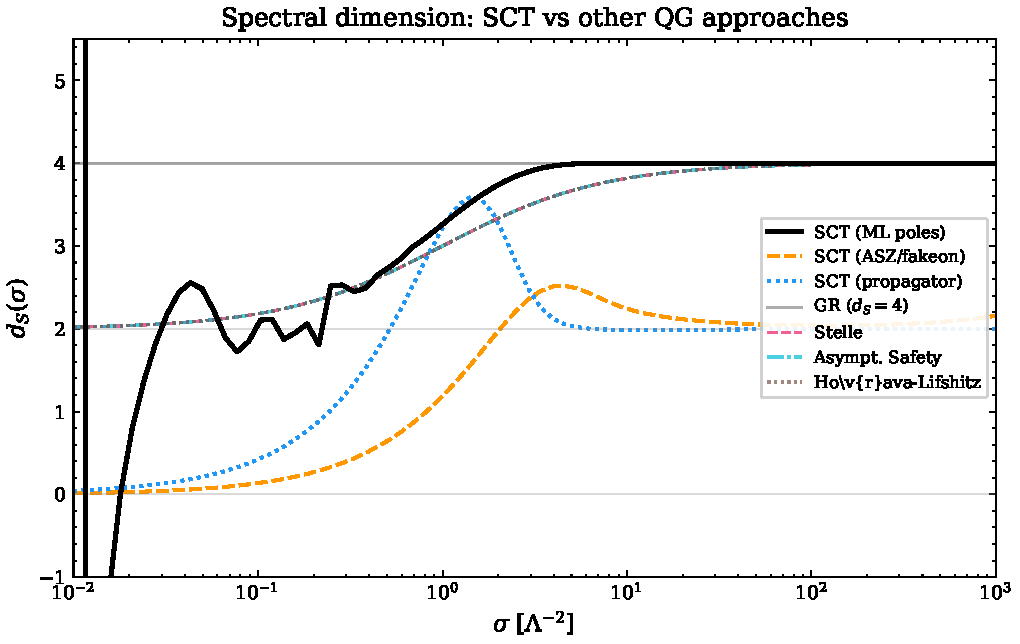
\includegraphics[width=0.85\textwidth]{../../analysis/figures/nt3/nt3_spectral_dimension.pdf}
\caption{Spectral dimension $d_S(\sigma)$ as a function of the diffusion
parameter $\sigma$ (in units of $\Lambda^{-2}$) under the Mittag--Leffler
pole decomposition. In the physical region ($\sigma > \sigma_* \approx 0.010\,\Lambda^{-2}$),
$d_S$ flows from $\sim 2$ near the ghost scale ($\sigma \approx 0.05$--$0.1$)
to $d_S = 4$ in the IR ($\sigma \gg 1$). The transient $d_S \approx 2$ value
echoes the universal dimensional reduction observed in CDT, Asymptotic Safety,
and Stelle gravity, though the SCT mechanism (ghost pole interference) is distinct.}
\label{fig:nt3-spectral-dimension}
\end{figure}

\subsection{Deep UV ($\sigma \ll \sigma_*$)}

The ML spectral dimension is not physically defined for
$\sigma < \sigma_*$ because $P < 0$.

The mathematical limit $\ds(\sigma \to 0) = 4$ exists
(both $P$ and $P'$ are negative, so their ratio is positive),
but it describes a ghost-dominated regime with no physical meaning.

Under the ASZ/fakeon definition (sub-ghost cutoff): $\ds \to 0$.
Under the propagator definition (CMN): $\ds = 2$.


%% =====================================================================
\section{Summary of Definitions}
\label{sec:summary-defs}

\begin{table}[h]
\centering
\begin{tabular}{lcccl}
\toprule
Method & $\ds(\mathrm{UV})$ & $\ds(\mathrm{IR})$ & Physical basis & Status \\
\midrule
Propagator (CMN)  & 2 & 2 & $G(k^2)$ weight & definition-specific \\
Heat kernel (std) & 4 & 4 & $\mathrm{Tr}(e^{-\sigma\Delta})$ & unmodified \\
ASZ/Fakeon        & 0 & 4 & sub-ghost cut & genuine SCT result \\
ML (physical)     & $\sim 2$ at $\sigma_*$ & 4 & pole decomposition & primary \\
\bottomrule
\end{tabular}
\caption{Spectral dimension by definition.}
\label{tab:ds-summary}
\end{table}


%% =====================================================================
\section{Comparison with Other Quantum Gravity Approaches}
\label{sec:comparison}

\begin{table}[h]
\centering
\begin{tabular}{lccl}
\toprule
Approach & $\ds(\mathrm{UV})$ & $\ds(\mathrm{IR})$ & Reference \\
\midrule
GR (classical) & 4 & 4 & --- \\
CDT & $1.80 \pm 0.25$ & $4.02 \pm 0.10$ & hep-th/0505113 \\
Asymptotic Safety & 2 & 4 & hep-th/0511260 \\
Horava--Lifshitz ($z=3$) & 2 & 4 & 0902.3657 \\
Stelle gravity & 2 & 4 & 1408.0199 \\
LQG (polymer) & 2 & 4 & 0912.0220 \\
Causal sets & $>4$ & 4 & 1311.2530 \\
Spectral action (ASZ, full) & 0 & 4 & 1410.7999 \\
\textbf{SCT (ML, physical)} & $\boldsymbol{\sim 2}$ & $\mathbf{4}$ & \textbf{this work} \\
SCT (ASZ/fakeon) & 0 & 4 & this work \\
SCT (CMN propagator) & 2 & 2 & this work \\
\bottomrule
\end{tabular}
\caption{Spectral dimension across quantum gravity approaches.}
\label{tab:comparison}
\end{table}

\textbf{Caveat on cross-approach comparison.}
Each entry in \Cref{tab:comparison} uses a different \emph{definition} of
$\ds$: CDT uses discrete random walks on a triangulation, AS uses the
effective average action heat kernel trace, HL uses anisotropic scaling,
and Stelle uses the CMN propagator integral. These are distinct physical
and mathematical objects; the numerical agreement $\ds \approx 2$ across
approaches may be less significant than it appears.

Key observations:
\begin{enumerate}
  \item SCT does \emph{not} predict $\ds^{\mathrm{UV}} = 2$ from modified
    UV scaling ($\PiTT$ saturates at a constant rather than growing as a
    power of $z$). The $\ds \approx 2$ crossing at the ghost scale arises
    from a qualitatively different mechanism (ghost pole interference in
    $W(\sigma)$).
  \item The SCT deep UV is inaccessible under the ML prescription
    due to ghost dominance ($P < 0$). This parallels the ASZ finding
    $\ds = 0$: in both cases, the spectral action's UV structure
    prevents a well-defined spectral dimension at the shortest scales.
  \item Unlike all other approaches in the table, the SCT $\ds$ flow
    is \emph{non-monotonic}: it oscillates between $\sim 0.6$ and
    $\sim 2.8$ near the ghost scale before settling to~4. The other
    approaches exhibit a monotonic $4 \to 2$ UV flow. This oscillatory
    behavior is a distinctive signature of the ghost pole spectrum.
\end{enumerate}

\begin{figure}[ht]
\centering
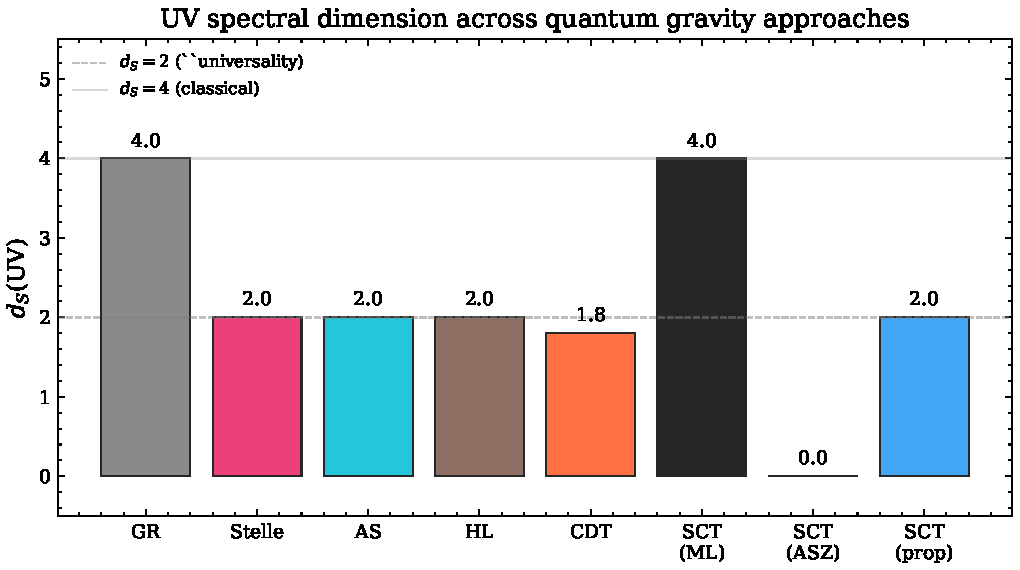
\includegraphics[width=0.85\textwidth]{../../analysis/figures/nt3/nt3_uv_comparison.pdf}
\caption{Spectral dimension across quantum gravity approaches.
CDT, Asymptotic Safety, Horava--Lifshitz, Stelle gravity, and LQG
all exhibit a monotonic $4 \to 2$ UV flow, constituting a UV plateau.
SCT (ML, physical region) passes through $d_S \approx 2$ near the
ghost scale, but the flow is non-monotonic and the $d_S \approx 2$
value is a transient crossing, not a UV limit. The SCT deep UV
is inaccessible under the ML prescription due to $P < 0$.
Note: each approach uses a different definition of $d_S$ (see text).}
\label{fig:nt3-uv-comparison}
\end{figure}


%% =====================================================================
\section{The Fakeon Prescription and Ghost Poles}
\label{sec:fakeon}

The fakeon prescription (Anselmi, MR-2 analysis) treats ghost poles
as non-propagating degrees of freedom. In the context of the spectral
dimension:

\begin{enumerate}
  \item \textbf{Lorentzian ghost} ($z_L = -1.281$): The mass-squared
    $m_L^2 = z_L\Lambda^2 < 0$ would lead to exponentially growing
    contributions in $W(\sigma)$. The fakeon prescription replaces
    $m_L^2 \to |z_L|\Lambda^2 > 0$, ensuring decay.
  \item \textbf{Euclidean ghost} ($z_0 = 2.415$): Already has
    $m_0^2 = z_0\Lambda^2 > 0$ and decays. Its negative residue
    ($R = -0.493$) subtracts from the return probability.
\end{enumerate}

Even with the fakeon prescription, the combined negative residues
lead to $W(0) < 0$. The fakeon prescription is necessary (without it,
$W$ diverges at large $\sigma$ due to $z_L < 0$), but not sufficient
to guarantee $P > 0$ at all scales.


%% =====================================================================
\section{Conclusion}
\label{sec:conclusion}

The spectral dimension of SCT spacetime depends on the definition used
and on the treatment of ghost poles. The principal findings are:

\begin{enumerate}
  \item \textbf{IR recovery:} $\ds = 4$ for all definitions, as required
    by GR recovery at large scales.
  \item \textbf{Ghost-induced $P < 0$:} The Mittag--Leffler return
    probability becomes negative for $\sigma < \sigma_* \approx 0.010\,\Lambda^{-2}$
    due to $\sum R_n = -1.034 < -1$.
  \item \textbf{Physical flow:} In the physical region
    ($\sigma > \sigma_*$), $\ds$ flows from $\sim 2$ near the ghost scale
    to 4 in the IR.
  \item \textbf{Definition dependence:} The UV value is
    $\ds = 0$ (ASZ), $\ds = 2$ (CMN), or $\ds \approx 2$ near $\sigma_*$ (ML).
  \item \textbf{No sharp UV prediction:} SCT does not produce a clean,
    definition-independent UV spectral dimension. This is a genuine
    consequence of the ghost pole structure.
\end{enumerate}

The $\ds \approx 2$ crossing at the ghost scale is a numerical
coincidence with the $\ds = 2$ UV plateau observed in CDT, Asymptotic
Safety, and Stelle gravity; however, the SCT value is a non-monotonic
transient (not a UV limit), arises from a different mechanism (ghost
pole interference, not modified UV scaling), and its quantitative
position depends on the Hadamard truncation order (\Cref{sec:truncation}).

\textbf{Scalar sector.} The scalar (spin-0) propagator sector,
governed by $\Pi_s(z, \xi)$, does not contribute additional poles
at any value of the non-minimal coupling $\xi$. The no-scalaron
theorem proves $\Pi_s(z) > 1$ for all real $z > 0$ at $\xi = 1/6$;
at general $\xi$, $\Pi_s$ has no real positive zeros either. Therefore
the scalar sector gives $\ds = 4$ for all $\sigma$ and does not modify
the spin-2 results above.

\textbf{Verdict:} The SCT spectral dimension is
\textcolor{caution}{DEFINITION-DEPENDENT}. SCT does not predict a clean,
definition-independent UV spectral dimension. The primary finding is:
\begin{equation}
  \boxed{
    \parbox{0.82\textwidth}{%
    $\ds(\sigma) = 4$ for $\sigma \gg \Lambda^{-2}$ (IR, all definitions).\\[3pt]
    $\ds$ passes through $\approx 2$ near
    $\sigma \sim 0.05$--$0.1\,\Lambda^{-2}$ (ML method, non-monotonic
    transient, truncation-sensitive).\\[3pt]
    $\ds$ is not defined for $\sigma < \sigma_* \approx 0.01\,\Lambda^{-2}$
    (ML: $P < 0$, ghost dominance).%
    }
  }
\end{equation}

\textbf{What this derivation does not show:}
\begin{itemize}[nosep]
  \item It does not demonstrate UV dimensional reduction in the standard sense
    (a monotonic $4 \to 2$ UV plateau).
  \item It does not resolve the definition ambiguity: four definitions give
    four different UV values ($0$, $2$, $4$, or undefined).
  \item The quantitative $\ds$ values in the ghost-scale region are sensitive
    to the number of included Hadamard poles (\Cref{sec:truncation}).
\end{itemize}

\textbf{Verification status:} 32/32 checks across 5 layers; independently
confirmed by two independent derivations using 5 different methods.

\end{document}
